
\documentclass[12pt]{article}
\usepackage{amsmath}
\usepackage{amsfonts}
\usepackage{mathrsfs}
\usepackage{lscape}
\usepackage{listings}
\usepackage{graphicx} % Allows for importing of figures
\usepackage{color} % Allows for fonts to be colored
\usepackage{comment} % Allows for comments to be made
\usepackage{accents} % Allows for accents to be made above and below text
%\usepackage{undertilde} % Allows for under tildes to take place for vectors and tensors
\usepackage[table]{xcolor}
\usepackage{array,ragged2e}
\usepackage{hyperref}
\usepackage{framed} % Allows boxes to encase equations and such
\usepackage{subcaption} % Allows for figures to be side-by-side
\usepackage{float} % Allows for images to not float in the document
\usepackage{booktabs}
%\usepackage[margin=0.75in]{geometry}
\usepackage[final]{pdfpages}
\usepackage{enumitem}
\usepackage[section]{placeins}

%%%%%%%%%%%%%%%%%%%%%%%%%  Function used to generate vectors and tensors %%%%%%%%%
\usepackage{stackengine}
\stackMath
\newcommand\tensor[2][1]{%
	\def\useanchorwidth{T}%
	\ifnum#1>1%
	\stackunder[0pt]{\tensor[\numexpr#1-1\relax]{#2}}{\scriptscriptstyle \sim}%
	\else%
	\stackunder[1pt]{#2}{\scriptscriptstyle \sim}%
	\fi%
}
%%%%%%%%%%%%%%%%%%%

\definecolor{mygrey}{rgb}{0.97,0.98,0.99}
\definecolor{codeblue}{rgb}{.2,0,1}
\definecolor{codered}{rgb}{1,0,0}
\definecolor{codegreen}{rgb}{0.3,0.33,0.12}
\definecolor{codegray}{rgb}{0.5,0.5,0.5}
\definecolor{codepurple}{rgb}{0.55,0.0,0.55}
\definecolor{codecyan}{rgb}{0.0,.4,.4}

\lstdefinestyle{mystyle}{
	backgroundcolor=\color{mygrey},   
	commentstyle=\color{codegreen},
	keywordstyle=\color{codeblue},
	stringstyle=\color{codepurple},
	numberstyle=\tiny\color{codegray},
	basicstyle=\footnotesize,
	breakatwhitespace=false,         
	breaklines=true,                 
	captionpos=b,                    
	keepspaces=true, 
	numbers=left,                    
	numbersep=5pt,                  
	showspaces=false,                
	showstringspaces=false,
	showtabs=false,                  
	tabsize=2
}
\lstset{style=mystyle}

\lstset{language=Matlab,backgroundcolor=\color{mygrey}}
\usepackage{lastpage}
\usepackage{fancyhdr}
\pagestyle{fancy}
%\lhead{\large{Nik Benko, John Callaway, Nick Dorsett, Martin Raming}} 
%\chead{\large{\textbf{ME EN 6960: Lab 1}}}
%\rhead{\today}
\cfoot{[\thepage\ of \pageref{LastPage}]}
\fancyheadoffset{.5cm}
\setlength{\parindent}{0cm}
\usepackage[left=.5in, right=0.50in, top=1.00in,bottom=1.00in]{geometry}
\usepackage{microtype} 
\usepackage{setspace}
\doublespace
%%%%%%%%%%%%%%%%%%%%%%%%%%%%%%%%%%%%%%%%%%%%%%%%%%%%%%%%%%%%%%%%%%%%%%%%%%
% git testing ii

\begin{document}
\title{ Determination of Dynamic Tensile Strength of Concrete Using a Split Hopkinson Pressure Bar  \\ \normalsize{ME EN 6960}}
\author{Nik Benko, John Callaway, Nick Dorsett, Martin Raming}
\maketitle

% Nik
\begin{abstract} 

\end{abstract}

\section{Introduction} % Nik
Accurate predictions of material failure are critical to the design of structures and mechanical devices. In order to make useful predictions of failure, material test conditions must replicate real-world loading scenarios as closely as possible. Standard material tests use application-specific test fixtures and specimen geometries to approximate the expected stress state i.e. tension, compression, shear, or combined loading. An additional, and often overlooked, aspect of the loading condition is the rate at which loads are applied. Many structures and devices are designed to be impacted at high enough speeds that the constitutive response of materials is significantly different from the material's quasi-static behavior. In these applications it is important to quantify a material's failure properties at high strain rates in order to determine if the use of the material is appropriate.  \\

In this report the high strain rate tensile behavior of concrete is investigated. Concrete is a very common material used in large structures such as buildings, bridges, and roadways, all of which may be subject to high strain rate loading. The compressive and tensile strengths of concrete have been shown to increase at high strain rates. The relationship between strain rate and compressive strength is relatively well established, while only few studies have investigated how the tensile strength of concrete changes with loading rate \cite{Jin2017}. A thorough understanding of this relationship may be able to further optimize structural design when high rate loading is expected. In order to load the brittle concrete samples in tension, a Flat Brazil Disc specimen is used.\\ 

A major challenge in dynamic material testing is accounting for the inertial effects of a rapidly moving loading apparatus. To overcome this challenge, Kolsky adapted a pressure bar technique originally used by Hopkinson to strike thin material specimens at high speeds\cite{Kolsky}. The long and thin bars of a Split-Hopkinson Pressure Bar (SHPB), combined with a thin material specimen, allow strain measurements from the bars to be analyzed with one dimensional wave analysis. This simplification of three dimensional mechanics down to a single dimension allows for the inertia of the striker bar to be accounted for.\\

An unaltered SHPB generates trapezoidal pulses, with sharp leading and trailing edges. This results in high frequency content in the incident pressure wave that creates inaccuracies in strain measurements and may be undesirable for certain material types. The two most common ways of addressing this issue is the use of pulse shaping, as proposed by Frew et al., and dispersion correction, demonstrated by Follansbee \cite{Frew2002} \cite{Follansbee}. Both methods were used in this investigation. In this report, the experimental apparatus, test protocol, data reduction, and data analysis methods are described in the methods section. A summary of the measured and reduced data is listed in the results section. The relation of these findings to the current literature are then discussed, and final conclusions are drawn. \\



\section{Methods}

\subsection{Experimental Techniques} 

\subsubsection {Split Hopkinson Pressure Bar} % Nick
%Gas gun, bar, location, etc
The SHPB system is built off of three main parts: the striker bar, the incident bar, and the transmitted bar as shown in Figure (bar alignment cartoon) \cite{Frew2002} \cite{Follansbee} \cite{Frew}. A gas gun was used to accelerate the striker bar into the incident bar and create a one-dimensional compression wave that travels down the incident bar \cite{Frew}. Upon reaching a test specimen placed at the end of the bar as in Figure \ref{fig:TestSetup}, the specimen is deformed at a very high strain rate by the compression wave \cite{Dai}. This deformation imparts a reaction force into the transmitted bar, creating a new compression wave. The remainder of the energy from the incident wave is reflected back along the incident bar as a tensile wave. The overall wavelength of the incident pulse is the length of the striker bar. Therefore, in order to fully measure both the incident and reflected pulses without interference between the two, the incident bar must be at least twice the length of the striker bar.
\\ \\
For a SHPB system to produce valid results, the stress wave must only propagate axially. For this assumption to be valid, several criteria must be met. The bars must be made from a homogeneous, isotropic material. Furthermore, the bars must be uniform in cross section, which is achieved through centerless grinding. Finally, initial impact must be kept low enough so that the elastic limit of the bar is not reached. It is also assumed that the stress distribution over the cross section of the bar must be uniform. This is not entirely accurate, but it has been proven that if the length of the bar is at least twenty times the diameter, the results are still acceptable. 
\\ \\
One of the limitations of a SHPB system is that with finite bars, dispersion effects must be considered due to variations in the speed different frequencies travel within a medium. Two methods are commonly used to compensate for dispersion. The first is the use of pulse shaping. Pulse shaping uses a sacrificial material placed between the striker bar and the incident bar. An ideal pulse shaper reduces the initial slope of the incident pulse so that it more closely resembles the specimen material response. By doing this, the high frequency content of the system is decreased and it can be assumed that only a few frequencies dominate the pulse. The second method of compensating for dispersion is through the use of post processing dispersion correction. Measurements are taken by strain gauges in the center of each bar to ensure that the incident and reflected waves are separately recorded. To then march these waveforms forward or backward in time to represent the conditions upon specimen failure, the Fourier series

\begin{equation}
F(n\Delta T) = \frac{A_0}{2} + \sum\limits_{k=1,2,...}^N [A_k cos(k \omega_0 n \Delta T - \phi_{TS}) + B_k sin(k\omega_0 n\Delta T - \phi_{TS})]
\end{equation}
is used, where 
\begin{align*}
\phi_{TS} =& k\omega_0(\Delta x/C_k) \\
A_0 =& \frac{2}{T} \int_0^T \! f(x) \, dt\\
A_k =& \frac{2}{T} \int_0^T \! f(t)cos(k\omega_0t) \, dt\\
B_k =& \frac{2}{T} \int_0^T \! f(t)sin(k\omega_0t) \, dt
\end{align*}

Here, $T$ is the period of the wave, $\omega_0$ is the fundamental frequency $\frac{2\pi}{T}$, $n$ = 1,2,...2$N$, where $N$ = half the number of recorded data points, $C_k$ is the speed of a wave at the $kth$ frequency, $\Delta T$ is the time step between recording intervals, and $\Delta x$ is the distance from the strain gauge to the specimen\cite{Gama}. Once the waves have been propagated so they are at the same point in time, the strain gauge readings can be translated into strain and force values can be determined. Force on the left side of the bar is found through the equation 

\begin{equation}
F_1 = A_{Bar}E_{Bar}(\varepsilon_I + \varepsilon_R)
\end{equation}

and similarly, force on the right side of the bar is

\begin{equation}
F_2 = A_{Bar}E_{Bar}(\varepsilon_T)
\end{equation}.

where $A_{Bar}$ is the area of the SHPB, $E_{Bar}$ is the elastic modulus of the SHPB, $\varepsilon_I$, $\varepsilon_T$ and $\varepsilon_R$ are the incident, transmitted and reflected strains. From force equilibrium, both of these force values should be the same. Finally, from ASTM D3957-08 (cite standard) the tensile strength of the Brazil disc specimens is found from

\begin{equation}
\sigma_t = \frac{2P}{\pi Dt}
\label{eq:stress}
\end{equation}

where $P$ is the force applied by one side of the bar, $t$ is the specimen thickness, and $D$ is the specimen diameter. Through the application of forces on the specimen geometry, the compression wave from the SHPB will produce a tensile loading to fail the specimen.

\subsubsection{High Strain Rate Data Acquisition} % Nick
%Strain gauges, scope
Data for the SHPB is recorded through strain gauges adhered to the center of each bar. These gauges are arranged in a full bride configuration which only measures deformations in the axial direction. This further helps satisfy the theoretical requirement for axial wave propagation because due to the difficulty in perfectly aligning the bars, other minute deformations may exist.
\\ \\
%Data was recorded through the use of a Dewetron (citation) data acquision system (DAQ). A very high sampling rate is desirable for the purposes of this experiment to get the 
In order to avoid aliasing a sample frequency equal to or greater than the Nyquist frequency ($f_N$) must be used \cite{Shukla} \cite{Sampling}. The Nyquist frequency is simply double the highest frequency component of the measured signal. Since high strain rates, as seen in the SHPB, result in high frequency components a very high sample rate is required. 

\subsubsection{Statistical Analysis} % John

Central tendency and dispersion are two common ways to quantify the distribution of a data set \cite{Shukla}. Central tendency is quantified using the measures of mean and median. The mean of a data set is given by
\begin{equation}
\bar{x} = \sum_{i=1}^{n}\frac{x_{i}}{n}
\end{equation}
where $\bar{x}$ is the mean, $n$ is the number of data points and $x_{i}$ is the ith data point. The median is the central value of an ordered set of the data. Dispersion represents the distribution of data around the central tendency, usually the mean. Dispersion is measured using standard deviation and variance, given by 
\begin{equation}
S_{x} = \left[\sum_{i=1}^{n}\frac{\left(x_{i}-\bar{x}\right)^2}{n-1}\right]^\frac{1}{2}
\end{equation}  
\begin{equation}
S_{x}^2 = \sum_{i=1}^{n}\frac{\left(x_{i}-\bar{x}\right)^2}{n-1}
\end{equation} 
where $S_{x}$ is the standard deviation and $S_{x}^2$ is the variance.

For experiments involving strength of materials due to brittle fracture, a Weibull distribution function can be applied to show the probability of failure at a given strength value \cite{Shukla}. The Weibull Distribution is given by
\begin{equation}
p(x) = 1-e^{-\left[\frac{\left(x-x_{o}\right)}{b}\right]^m} \text{ for } x > x_{o}
\end{equation}
\begin{equation}
p(x) = 0  \text { for } x < x_{o}
\end{equation} 
where $p(x)$ is the probability of failure occurring at $x$, $x_{o}$ is the zero strength value of the distribution, $b$ is scale parameter and $m$ is the Weibull slope parameter. The values of distribution parameters $x_{o}$, $b$ and $m$ can be determined iteratively or by use of a commercial software such as MATLAB. MATLAB has a built in function, $wblfit$. that generates the Weibull parameters and probability distribution function with a 95\% confidence interval (ref).

\subsection{Procedure} % John

Concrete Brazil Disc specimens with a diameter of 19.05 mm and thickness of 6.35 mm were loaded in a SHPB test setup. The SHPB utilized 19.05 mm diameter aluminum 7075-T6 bars for the incident and transmitted bars. The incident bar length was 2.438 m and the transmitted bar length was 1.930 m. Aluminum platens with a matching acoustic impedance were attached to the loading end of the incident and transmitted bars to prevent damage to the SHPB apparatus from the concrete specimens. A 1.058 mm thick, 9.525 mm diameter lead pulse shaper was placed on the non-loading end of the incident bar for each test. The striker bar was propelled using a REL gas gun. The experimental setup can be seen in Figure \ref{fig:TestSetup}.
\\ \\
Initial calibration and bar wave speed were determined without specimens using a gas gun pressure of 10.2 psi. A total of ten specimens were tested at four separate gas gun pressures - 8, 9, 10.2 and 12.4 psi. Strain gauges attached to both the incident and transmitted bars were used to detect the incident, reflected and transmitted waves in the bar. The strain gauges were located 1.219 m from the loading point on the incident bar and 0.965 m from the loading point on the transmitted bar. Voltage outputs from the strain gauges were collected using a Tektronix DPO 2004B oscilloscope. All analysis was completed in MATLAB.   

\subsection{Error and Uncertainties} % Nick 

The main source of uncertanty in the experiment was in the data analysis. It has been shown that the data is very sensitive to the exact value of $C_0$ as well as in shifting the pulse through time \cite{Gama}. In our data analysis, the wave speed was determined from a calibration experiment. However, force equilibrium was not satisfied, likely due to errors in shifting the incident and/or reflected waves.
%this is the only even remotely quantificable source of error I could think of

\section{Results} % John

Thirty five concrete Brazil Disc specimens produced a mean dynamic tensile strength of 15.77 MPa, with a median of 15.18 MPa and standard deviation of 3.60 MPa. The data was found to fit a Weibull distribution with $x_{o}$ = 7.84 MPa, $b$ = 17.18 MPa and $m$ = 4.9951. A Weibull Probability Distribution Function plot was create to verify the Weibull distribution parameters and is presented in Figure \ref{fig:Weibull}. A comparison of the gas gun pressure and dynamic tensile strength of concrete showed no relationship, which is visualized in Figure \ref{fig:GasGun}.

\section{Discussion} % Martin
Inorder to calculate $\sigma_t$ in Equation \ref{eq:stres} we assumed force homogenization, therefor only $F_2$ was used. The results of these calculations show a higher ultimate tensile strength than that of quasi-static experiments. This observation of strain rate dependence is consistent with work done by others, such as D.L. Grote et al. \cite{Grote}. Although this experiment did not find a relationship of gas gun pressure to ultimate tensile strengths it would seem there is a relationship  between strain rate and ultimate tensile strength. This could be due gas gun pressure effects on strain rate being undetermined. 
\\
\\
The pulse shaper as mentioned previously was chosen based on the lower rise of the generated pulse when compared to pulses created using other pulse shapers as shown in Figure \ref{fig:pulseshaper}. By using a pulse shaper a value of 50 was used for $N$ instead of $f_N$ as suggested by Li and Lambros \cite{Li} to aid in computation time with out loss of accuracy.
\\
\\
When performing a statistical analysis not all data was used.  The date chosen for removal was based around the code used for data reduction utilizes the initial rise to mark the point at which to begin analysis..  Samples 11, 31, and 32 were left out of the analysis as these samples were missing data for the initial rise of the pulse on the incident bar and   Samples 39-46 were also removed for similar reasons.  Instead of an incomplete data set these samples have multiple waves beyond the  reflected incident wave.
\\
\\
T


\section{Conclusion} % Nik

% Bar speed and strain rate % Martin
% Forward and backward propogation of waves % Nick
% Conversion of voltage to strain, strain to force, force to strength % Nick
% Statistical Analysis % John

\section{Figures}
\begin{figure}[H]
	\centering
	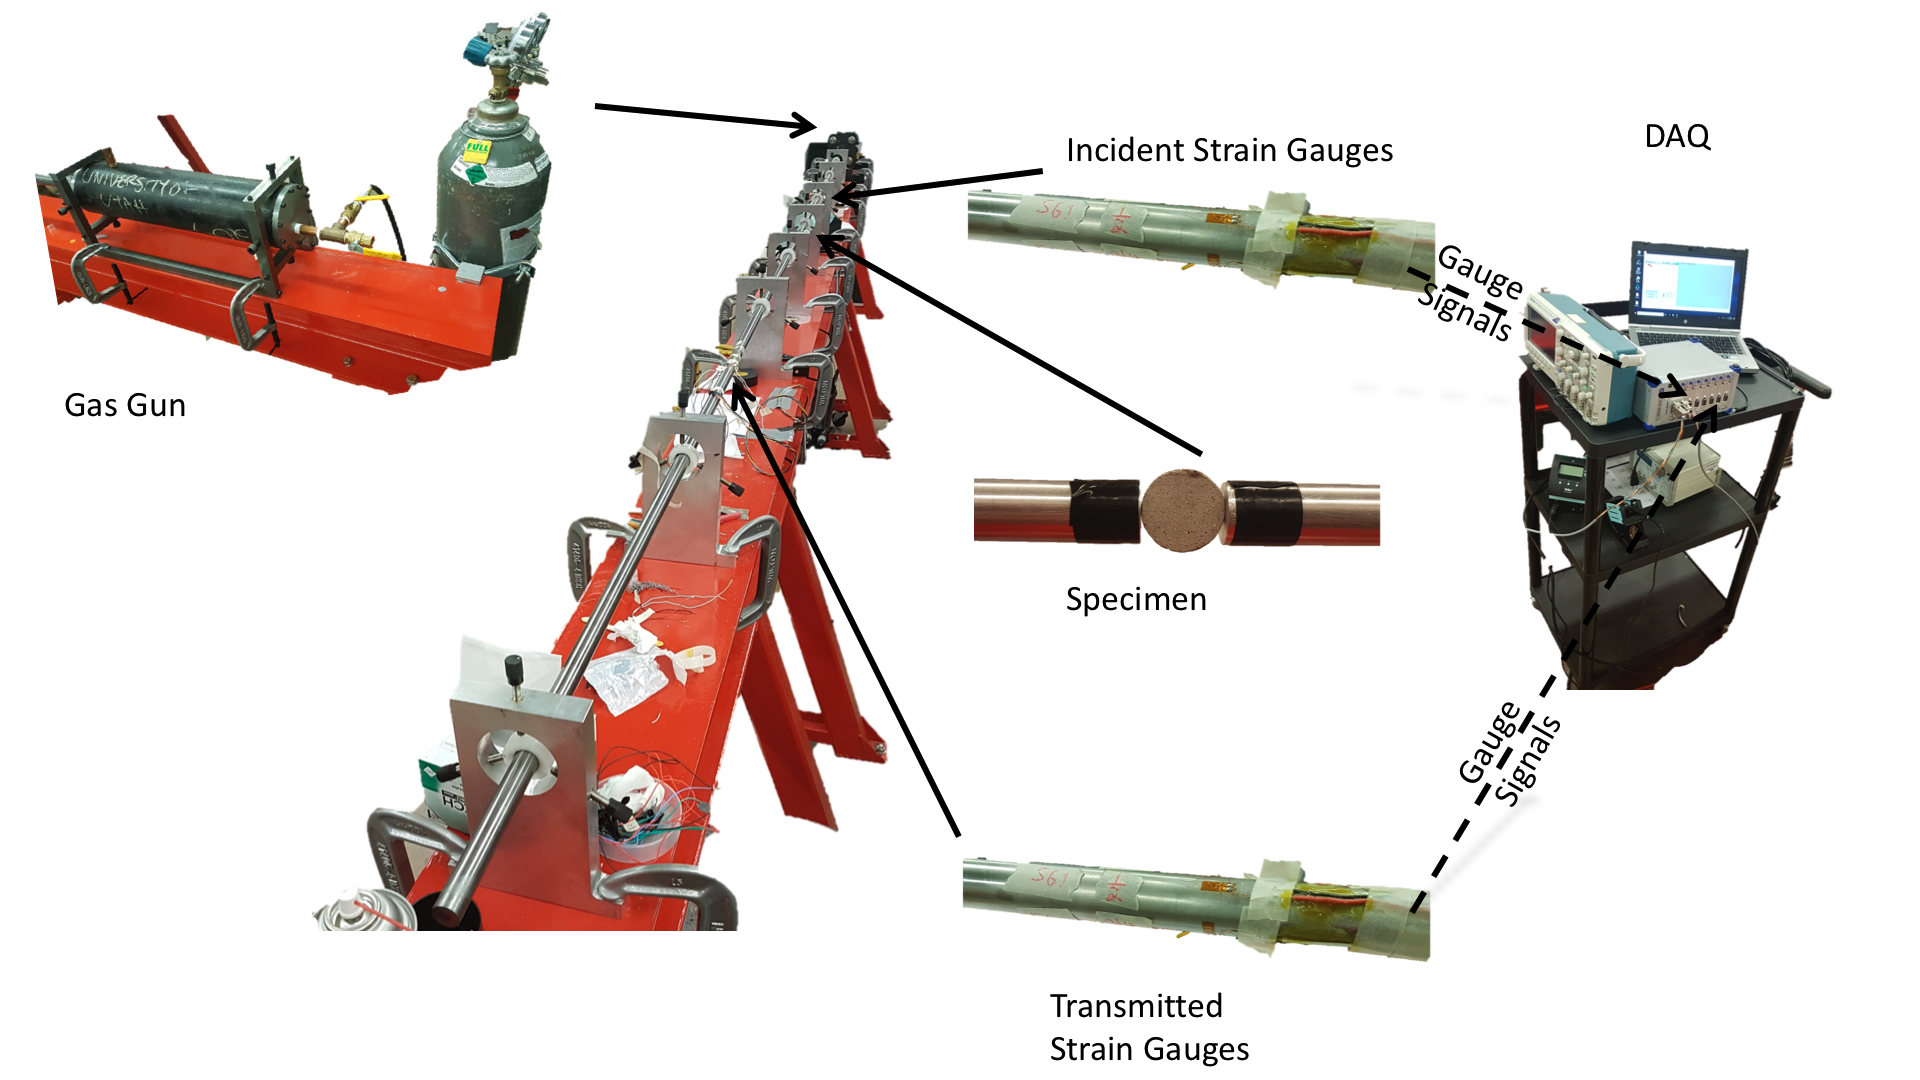
\includegraphics[width=1\textwidth]{TestSetUp.png}
	\caption{Experimental setup of the Split Hopkinson Pressure Bar}
	\label{fig:TestSetup}
\end{figure}

\begin{figure}[H]
	\centering
	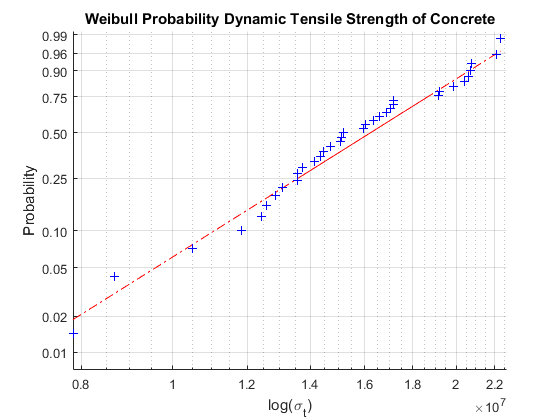
\includegraphics[width=0.67\textwidth]{Weibull.png}
	\caption{Weibull Probability Distribution Function plot of concrete Brazil Disc specimens}
	\label{fig:Weibull}
\end{figure}

\begin{figure}[H]
	\centering
	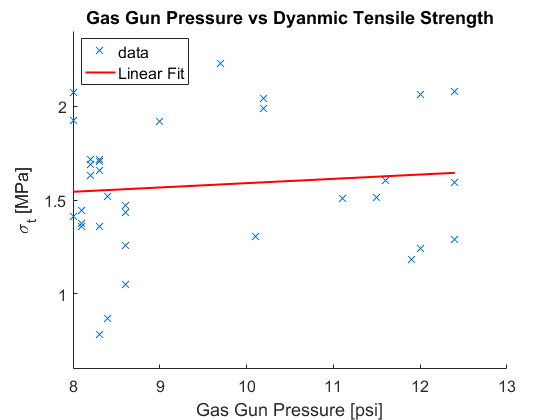
\includegraphics[width=0.67\textwidth]{Pressure_TensileStrength.png}
	\caption{Comparison of Gas Gun Pressure and Calculated Dynamic Tensile Strength of Concrete}
	\label{fig:GasGun}
\end{figure}

\begin{figure}[H]
	\centering
	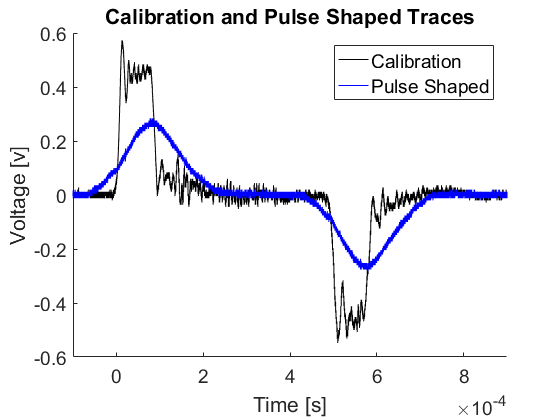
\includegraphics[width=1\textwidth]{pulseshaper.png}
	\caption{Calibration wave form and  comparison of the waveforms generated by use of different pule shapers with the bars apart.}
	\label{fig:pulseshaper}
\end{figure}

\section{Tables}
%Recoded Experimental Data:
%\begin{table}[h]\footnotesize
%	\centering
%	\begin{tabular}{ |l|l|l|l| }
%		\hline
%		\multicolumn{2}{|c|}{\textbf{Mode I}}&\multicolumn{2}{|c|}{\textbf{Mixed Mode}}\\ \hline
%		\textbf{Load [N]} & \textbf{Image Number}&\textbf{Load [N]} & \textbf{Image Number}\\  \hline
%		0-5 & 7.784 & 0-4 & 25.58 \\ \hline
%		6& 7.784 & 5 & 27.58 \\ \hline
%		7 & 93.77 & 6 & 86 \\ \hline
%		8 & 215.6 & 7 &191.7 \\ \hline
%		9 & 295 & 8 & 324 \\ \hline
%		10 & 412 & 9 & 431 \\ \hline
%		11 & 489.6 & 10 & 486 \\ \hline
%		12 & 587 & 11 & 534.7 \\ \hline
%		13 & 745 & 12 & 629.1 \\ \hline
%		14 & 834 & 13 & 761.7 \\ \hline
%		15 & 899 & 14 & 805.3 \\ \hline
%		16 & 952 & 15 & 849.6 \\ \hline
%		17 & 1010 & 16 & 896 \\ \hline
%		-	& - & 17 & 1000 \\ \hline
%		
%		
%		
%	\end{tabular}
%	\caption{Loads and associated image number, first few images were used as reference images.}
%	\label{tab:data}
%\end{table}
%% All layups
%\
%\section{Appendix}
%
%%\subsection{Code}
%%
%%\begin{verbatim}
%%
%%\end{verbatim}
%
%\newpage
\bibliographystyle{IEEEtran}
\bibliography{Lab3Bib}
\end{document}